\let\negmedspace\undefined
\let\negthickspace\undefined
\documentclass[journal]{IEEEtran}
\usepackage[a5paper, margin=10mm, onecolumn]{geometry}
%\usepackage{lmodern} % Ensure lmodern is loaded for pdflatex
\usepackage{tfrupee} % Include tfrupee package

\setlength{\headheight}{1cm} % Set the height of the header box
\setlength{\headsep}{0mm}     % Set the distance between the header box and the top of the text

\usepackage{gvv-book}
\usepackage{gvv}
\usepackage{cite}
\usepackage{amsmath,amssymb,amsfonts,amsthm}
\usepackage{algorithmic}
\usepackage{graphicx}
\usepackage{textcomp}
\usepackage{xcolor}
\usepackage{txfonts}
\usepackage{listings}
\usepackage{enumitem}
\usepackage{mathtools}
\usepackage{gensymb}
\usepackage{comment}
\usepackage[breaklinks=true]{hyperref}
\usepackage{tkz-euclide} 
\usepackage{listings}
\usepackage{gvv}                                        
\def\inputGnumericTable{}                                 
\usepackage[latin1]{inputenc}                                
\usepackage{color}                                            
\usepackage{array}                                            
\usepackage{longtable}                                       
\usepackage{calc}                                             
\usepackage{multirow}                                         
\usepackage{hhline}                                           
\usepackage{ifthen}                                           
\usepackage{lscape}
\usepackage{circuitikz}
\tikzstyle{block} = [rectangle, draw, fill=blue!20, 
    text width=4em, text centered, rounded corners, minimum height=3em]
\tikzstyle{sum} = [draw, fill=blue!10, circle, minimum size=1cm, node distance=1.5cm]
\tikzstyle{input} = [coordinate]
\tikzstyle{output} = [coordinate]


\begin{document}

\bibliographystyle{IEEEtran}
\vspace{3cm}

\title{1.5.36}
\author{EE25BTECH11049 - Sai Krishna Bakki}
 \maketitle
% \newpage
% \bigskip
{\let\newpage\relax\maketitle}

\renewcommand{\thefigure}{\theenumi}
\renewcommand{\thetable}{\theenumi}
\setlength{\intextsep}{10pt} % Space between text and floats


\numberwithin{equation}{enumi}
\numberwithin{figure}{enumi}
\renewcommand{\thetable}{\theenumi}

\textbf{Question}:\\
Point P\brak{x,4} lies on the line segment joining the points $\vec{A}$\brak{-5, 8} and $\vec{B}$\brak{4,-10}. Find the ratio in which point P divides the line segment AB. Also, find the value of x. \\ 
\solution \\
Let 
\begin{align}
\vec{A}= \myvec{-5 \\ 8}, \vec{B}= \myvec{4 \\ -10} , \vec{P} = \myvec{x \\ 4}
\end{align}    

Since $\vec{P}$ lies on $\vec{A}$ and $\vec{B}$, they must be collinear
\begin{align}
\therefore \text{rank}\myvec{\vec{B} - \vec{A} & &\vec{P} - \vec{A}} = 1
\end{align}
\begin{align}
    \text{rank}\myvec{9 & x+5 \\ -18 & -4} = 1
\end{align}
\begin{align}
	\myvec{9 &  x+5\\ -18 & -4} \xleftrightarrow[]{R_2 \rightarrow {2R_1 + R_2}} \myvec{9 & x+5 \\ 0 & 2x+6}  
\end{align}
The number of non zero rows in the row reduced matrix (also known as {\em echelon form}) is defined as the rank. For above matrix to be of rank 1,
\begin{align}
    2x+6 = 0
\end{align}
\begin{align}
\therefore x = -3
\end{align}
Thus $\vec{P}$ is :	
\begin{align}
    \vec{P} = \myvec{-3 \\ 4}
\end{align}

let $\vec{P}$ divide the line joining points $\vec{A}$ and $\vec{B}$ in the ratio $k:1$.

\begin{align}
    \vec{P}=\frac{k\vec{B+\vec{A}}}{k+1}
\end{align}

\begin{align}
    k\brak{\vec{P}- \vec{B}} = \vec{A}-\vec{P}
k=\frac{\brak{\vec{P}-\vec{B}}^T\brak{\vec{A}-\vec{P}}}{||\brak{\vec{P}-\vec{B}}||^2}    
\end{align}

\begin{align}
    k=\frac{\myvec{x-4 \\ -14} \cdot \myvec{-5-x\\4}}{{\norm{\myvec{x-4 \\ -14}}}^2}
\end{align}

substituting the value of $x$ as , we get the value of $k$ as

\begin{align}
    k=2/7
\end{align}

\begin{figure}[H]
    \centering
    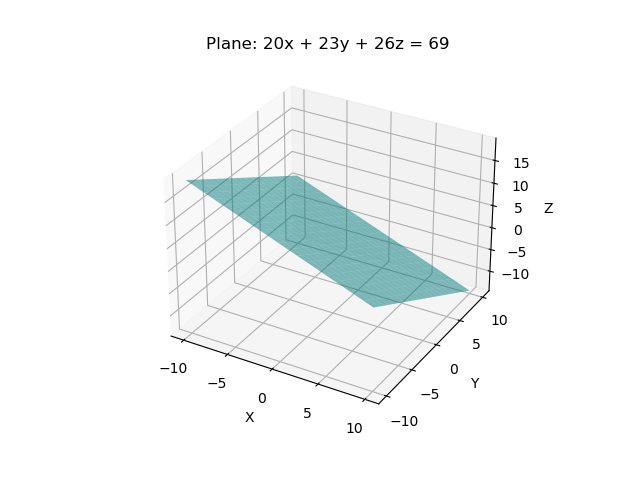
\includegraphics[width=0.6\columnwidth]{figs/Figure.png}
\end{figure}

\begin{figure}[H]
    \centering
    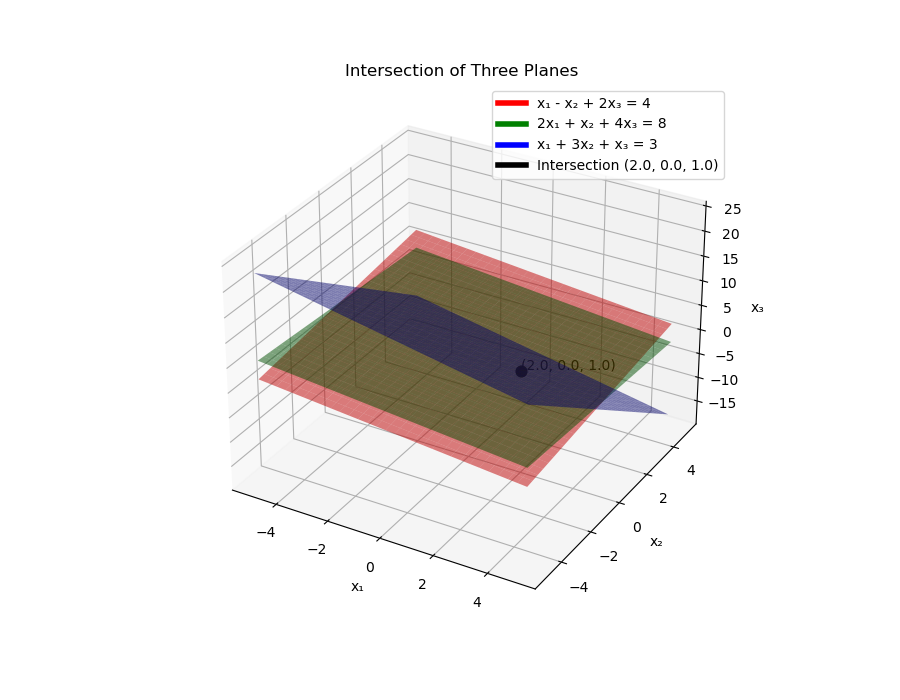
\includegraphics[width=0.6\columnwidth]{figs/Figure_1.png}
\end{figure}
\end{document}
